{\Large \textbf{How to...} \par}

\begin{description}
 	\item[get a license?] \hfill \\
 		As this is free software, there is no need to buy any licenses. To use this software, simply 
		sign up for a UserName on the website, Log In, and make use of the shuffling system.
 		\begin{figure}[H] 
		 	\centering
			 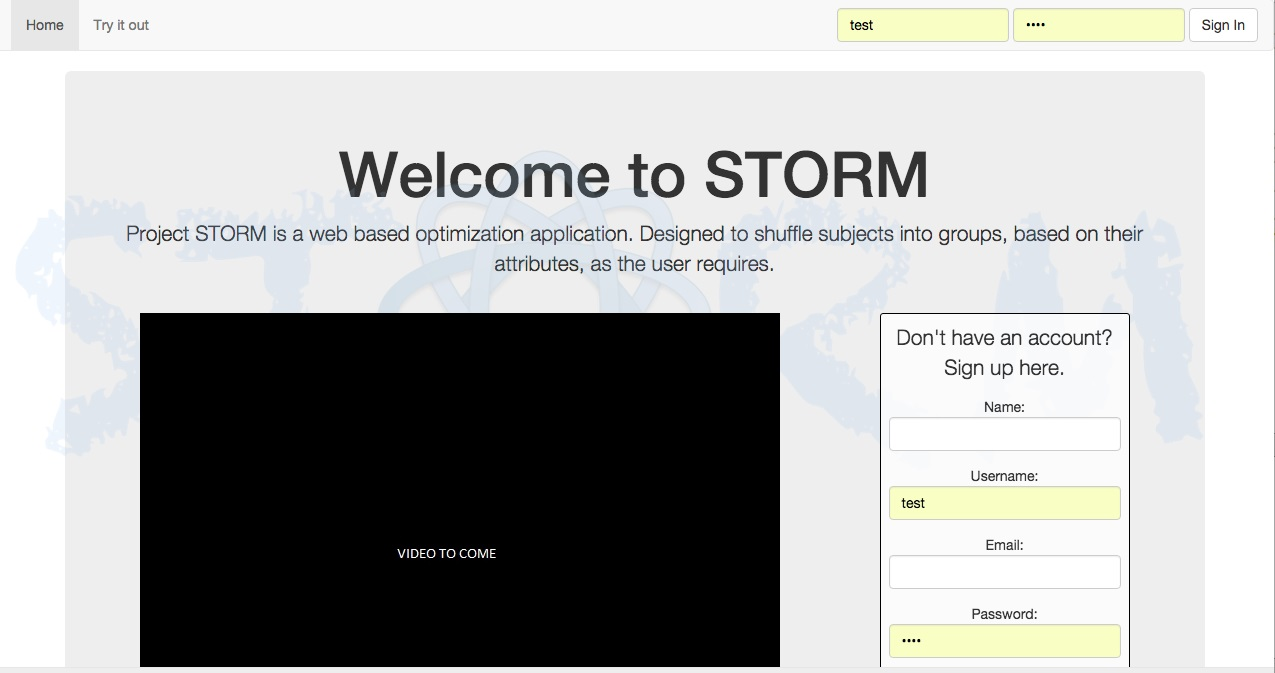
\includegraphics[width=13cm]{./graphics/HomePage.jpg}
			 \caption{STORM Homepage}
		 \end{figure}
 	\item[get a User ID] \hfill \\
		To sign up for an account, and get a User ID, enter user details in the appropriate fields in the 		following figure.\par
		 \begin{figure}[H] 
		 \centering
		 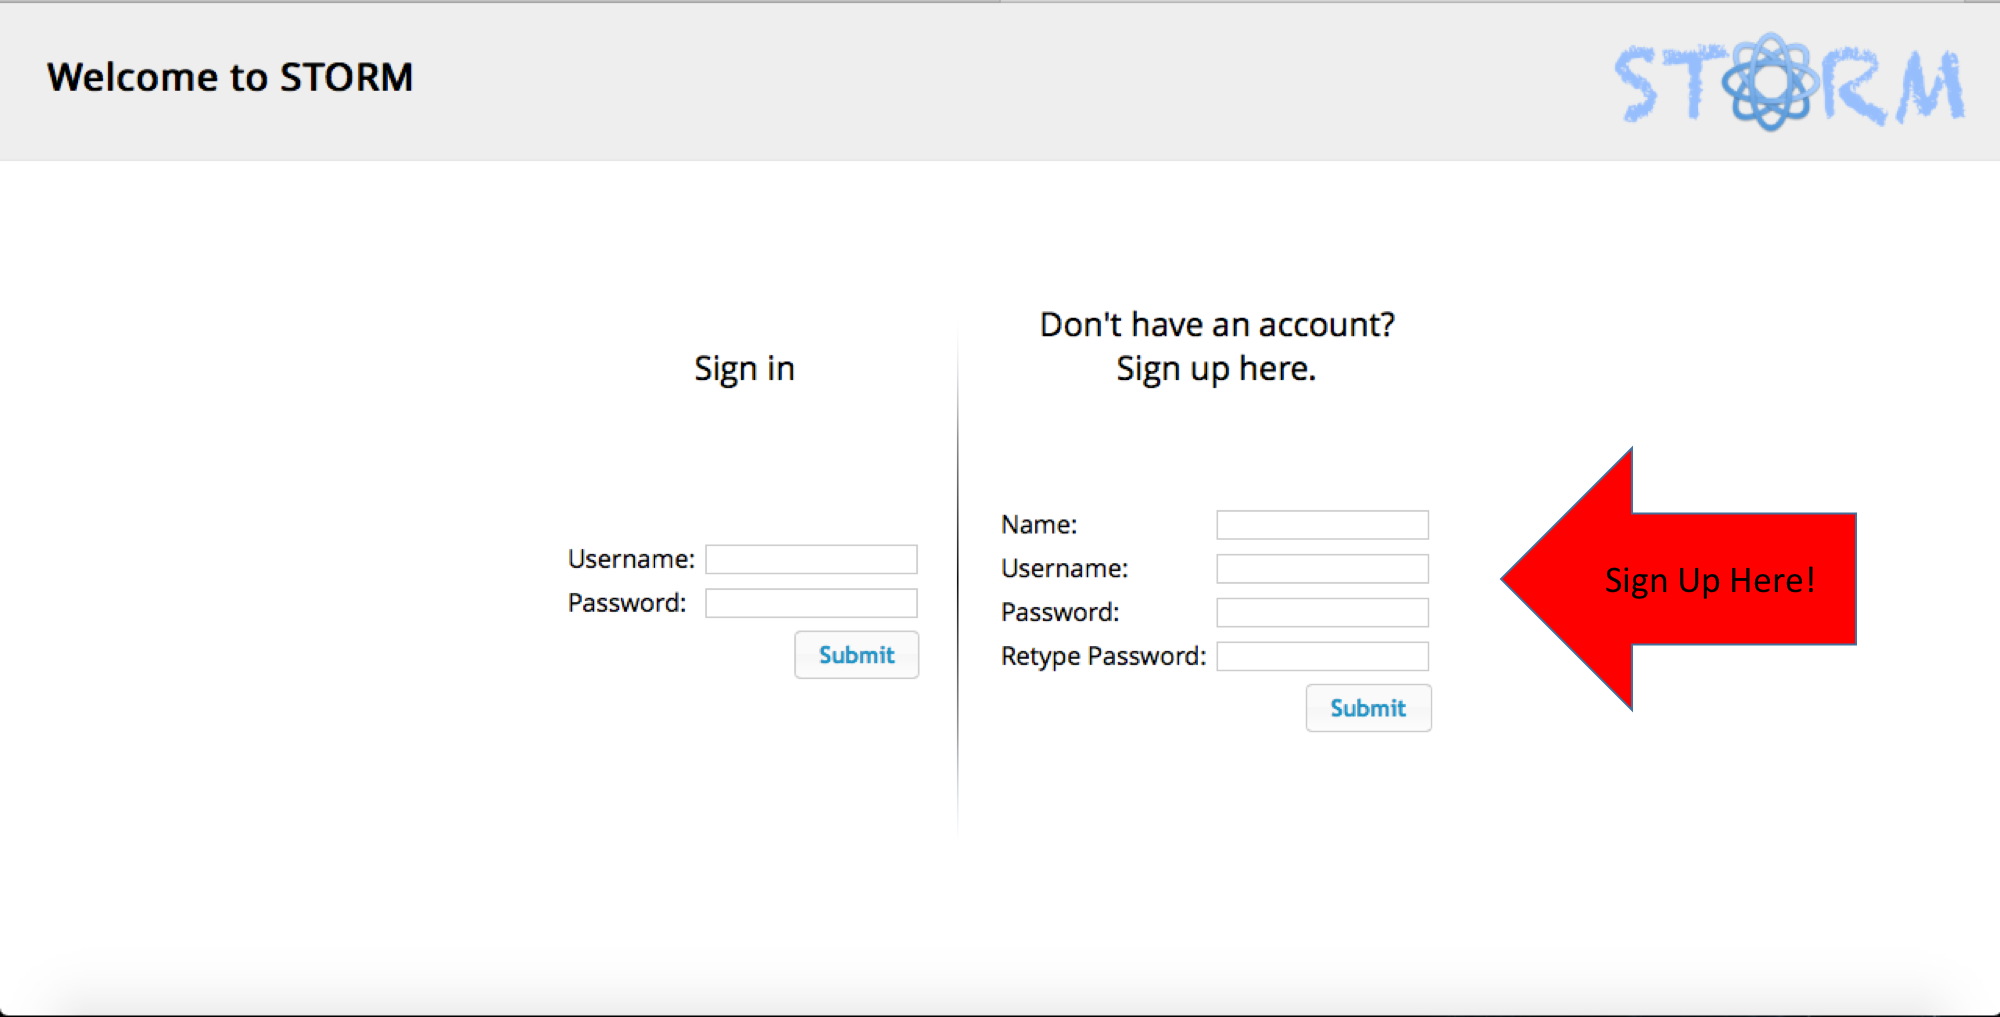
\includegraphics[width=6cm]{./graphics/StormUMSU1.jpg}
		 \caption{Signing Up to STORM}
		 \end{figure}
   		Click on submit and the system will register the user in the database.
	\item[log in] \hfill \\
 		To log in to an account, enter user details in the appropriate fields in the following figure.\par
   		\begin{figure}[H] 
		\centering 
		
\includegraphics[width=10cm]{./graphics/StormUMSU2.jpg}
		\caption{Logging In to STORM}
		\end{figure}
   		Click on submit and the system will navigate to the user's specific team shuffling page.
    	\item[change Username] \hfill \\
 		"Place Holder"
	\item[change password] \hfill \\
 		"Place Holder"
	\item[use the system as a guest] \hfill \\
 		Guests to the system will be able to access the website, and navigate around to see what it
		is all about, without having to log in or register and start shuffling teams from the first foot in 		the door. To access this feature, just navigate to the homepage, and click on "See how it 			works" as indicated in the Figure below.\par
		\begin{figure}[H] 
		\centering  
		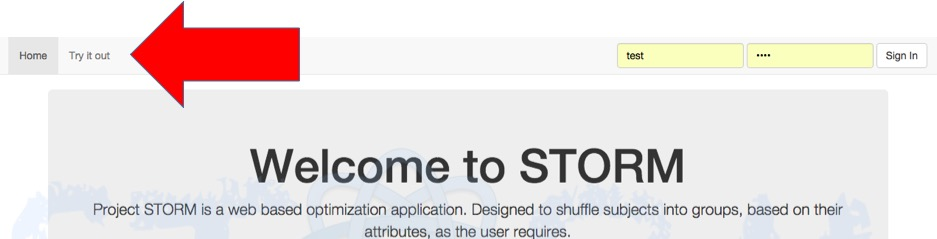
\includegraphics[width=10cm]{./graphics/TryOut.jpg}
		\caption{Using STORM as a guest}
		\end{figure}
				
\end{description}